\documentclass[11pt]{article}
\usepackage[textwidth=18.0cm, textheight=23.0cm, top=2.0cm]{geometry}
\usepackage{pst-all}
\usepackage{amssymb}
\usepackage{tikz}
\usepackage{underscore}\begin{document}
\pagestyle{empty}


ClassName: \underline{\textbf{Class_10.2bp-23}}
\par
BinSize: \underline{\textbf{100 × 100}}
\par
ReduceSize: \underline{\textbf{100 × 100}}
\par
TypeNum: \underline{\textbf{60}}
\par
Num: \underline{\textbf{60}}
\par
OutS: \underline{\textbf{80000}}
\par
InS: \underline{\textbf{69409}}
\par
Rate: \underline{\textbf{0.868}}
\par
UB: \underline{\textbf{8}}
\par
LB0: \underline{\textbf{7}}
\par
LB: \underline{\textbf{8}}
\par
LBWithCut: \underline{\textbf{8}}
\par
NodeCut: \underline{\textbf{0}}
\par
ExtendedNodeCnt: \underline{\textbf{1}}
\par
GenNodeCnt: \underline{\textbf{1}}
\par
PrimalNode: \underline{\textbf{0}}
\par
ColumnCount: \underline{\textbf{48}}
\par
TotalCutCount: \underline{\textbf{0}}
\par
RootCutCount: \underline{\textbf{0}}
\par
LPSolverCnt: \underline{\textbf{41}}
\par
PricingSolverCnt: \underline{\textbf{41}}
\par
BranchAndBoundNum: \underline{\textbf{1}}
\par
isOpt: \underline{\textbf{false}}
\par
TimeOnInitSolution: \underline{\textbf{600.000 s}}
\par
TimeOnPrimal: \underline{\textbf{0.000 s}}
\par
TimeOnPricing: \underline{\textbf{2999.669 s}}
\par
TimeOnRmp: \underline{\textbf{0.093 s}}
\par
TotalTime: \underline{\textbf{3600.012 s}}
\par
\newpage


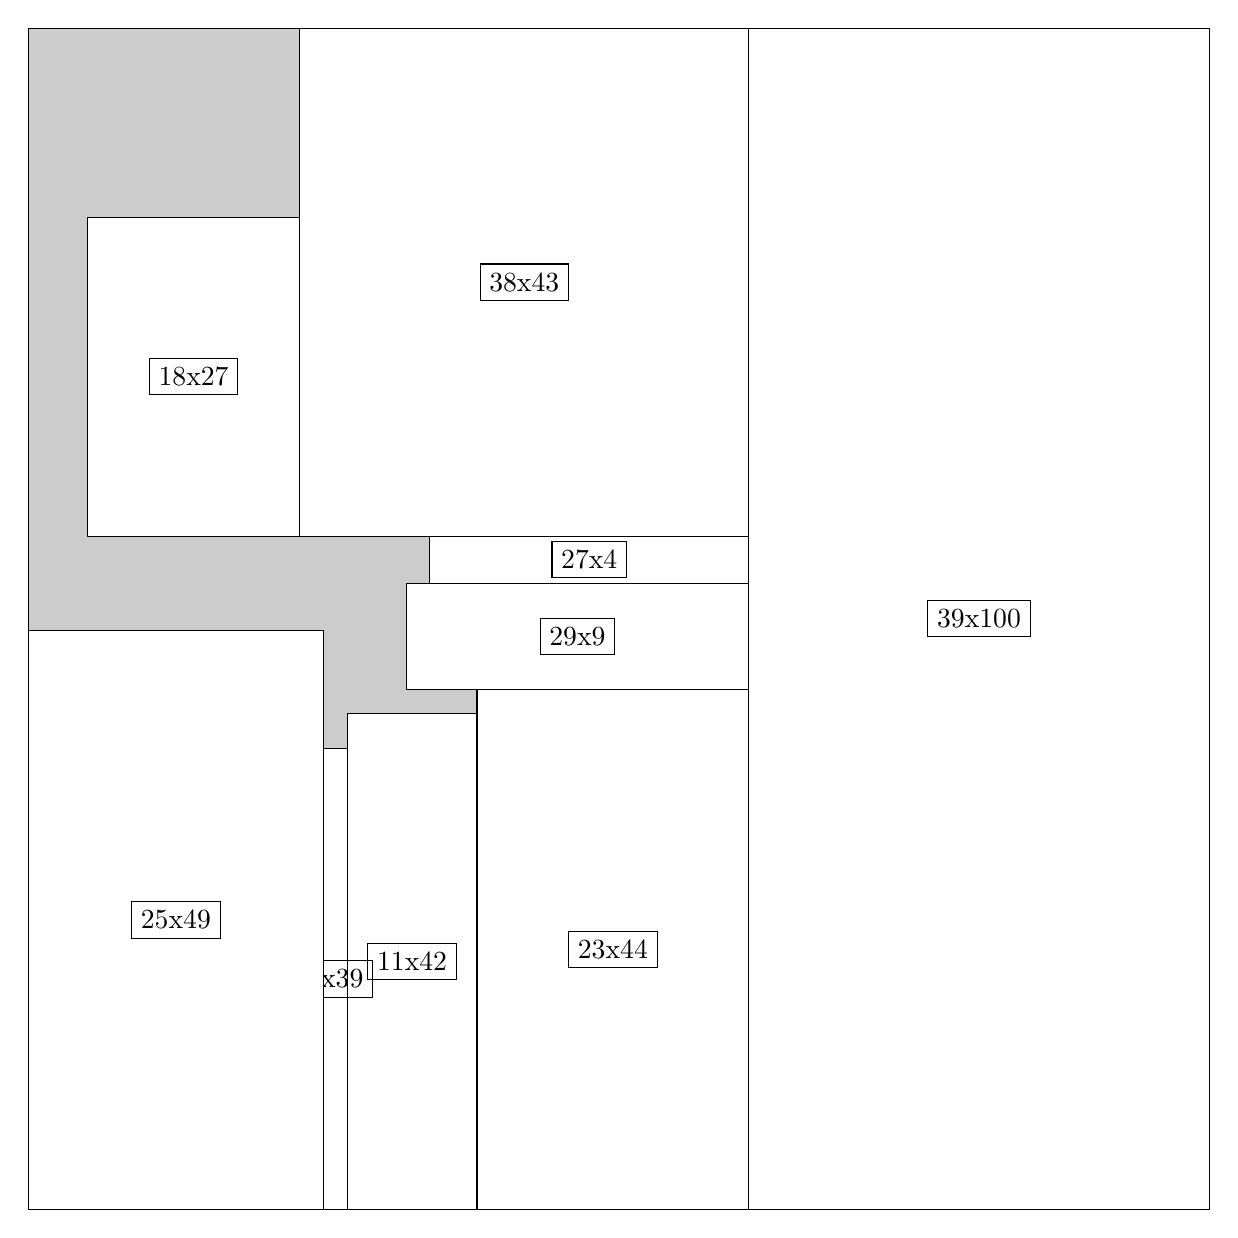
\begin{tikzpicture}[shorten >=1pt,scale=1.0,every node/.style={scale=1.0},->]
\tikzstyle{vertex}=[circle,fill=black!25,minimum size=14pt,inner sep=0pt]
\filldraw[fill=gray!40!white, draw=black] (0,0) rectangle (15.0,15.0);
\foreach \name/\x/\y/\w/\h in {39x100/9.15/0.0/5.85/15.0,23x44/5.7/0.0/3.4499999999999997/6.6,11x42/4.05/0.0/1.65/6.3,2x39/3.75/0.0/0.3/5.85,29x9/4.8/6.6/4.35/1.3499999999999999,27x4/5.1/7.949999999999999/4.05/0.6,25x49/0.0/0.0/3.75/7.35,38x43/3.4499999999999997/8.549999999999999/5.7/6.45,18x27/0.75/8.549999999999999/2.6999999999999997/4.05}
\filldraw[fill=white!40!white, draw=black] (\x,\y) rectangle node[draw] (\name) {\name} ++(\w,\h);
\end{tikzpicture}


w =39 , h =100 , x =61 , y =0 , v =3900
\par
w =23 , h =44 , x =38 , y =0 , v =1012
\par
w =11 , h =42 , x =27 , y =0 , v =462
\par
w =2 , h =39 , x =25 , y =0 , v =78
\par
w =29 , h =9 , x =32 , y =44 , v =261
\par
w =27 , h =4 , x =34 , y =53 , v =108
\par
w =25 , h =49 , x =0 , y =0 , v =1225
\par
w =38 , h =43 , x =23 , y =57 , v =1634
\par
w =18 , h =27 , x =5 , y =57 , v =486
\par
\newpage


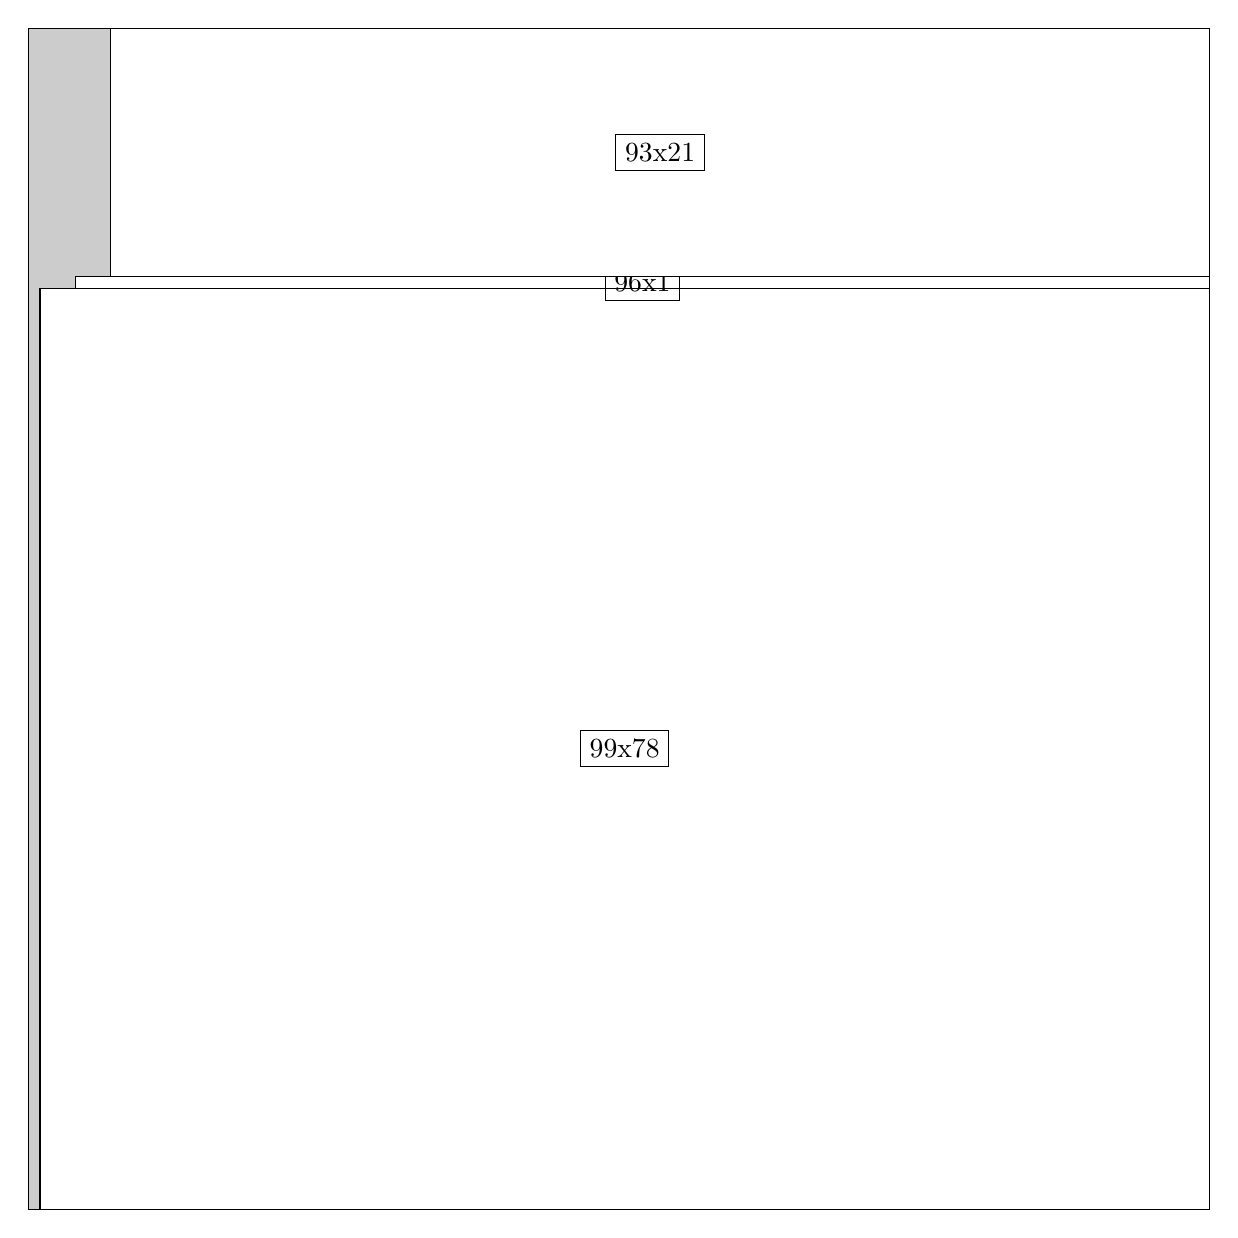
\begin{tikzpicture}[shorten >=1pt,scale=1.0,every node/.style={scale=1.0},->]
\tikzstyle{vertex}=[circle,fill=black!25,minimum size=14pt,inner sep=0pt]
\filldraw[fill=gray!40!white, draw=black] (0,0) rectangle (15.0,15.0);
\foreach \name/\x/\y/\w/\h in {99x78/0.15/0.0/14.85/11.7,96x1/0.6/11.7/14.399999999999999/0.15,93x21/1.05/11.85/13.95/3.15}
\filldraw[fill=white!40!white, draw=black] (\x,\y) rectangle node[draw] (\name) {\name} ++(\w,\h);
\end{tikzpicture}


w =99 , h =78 , x =1 , y =0 , v =7722
\par
w =96 , h =1 , x =4 , y =78 , v =96
\par
w =93 , h =21 , x =7 , y =79 , v =1953
\par
\newpage


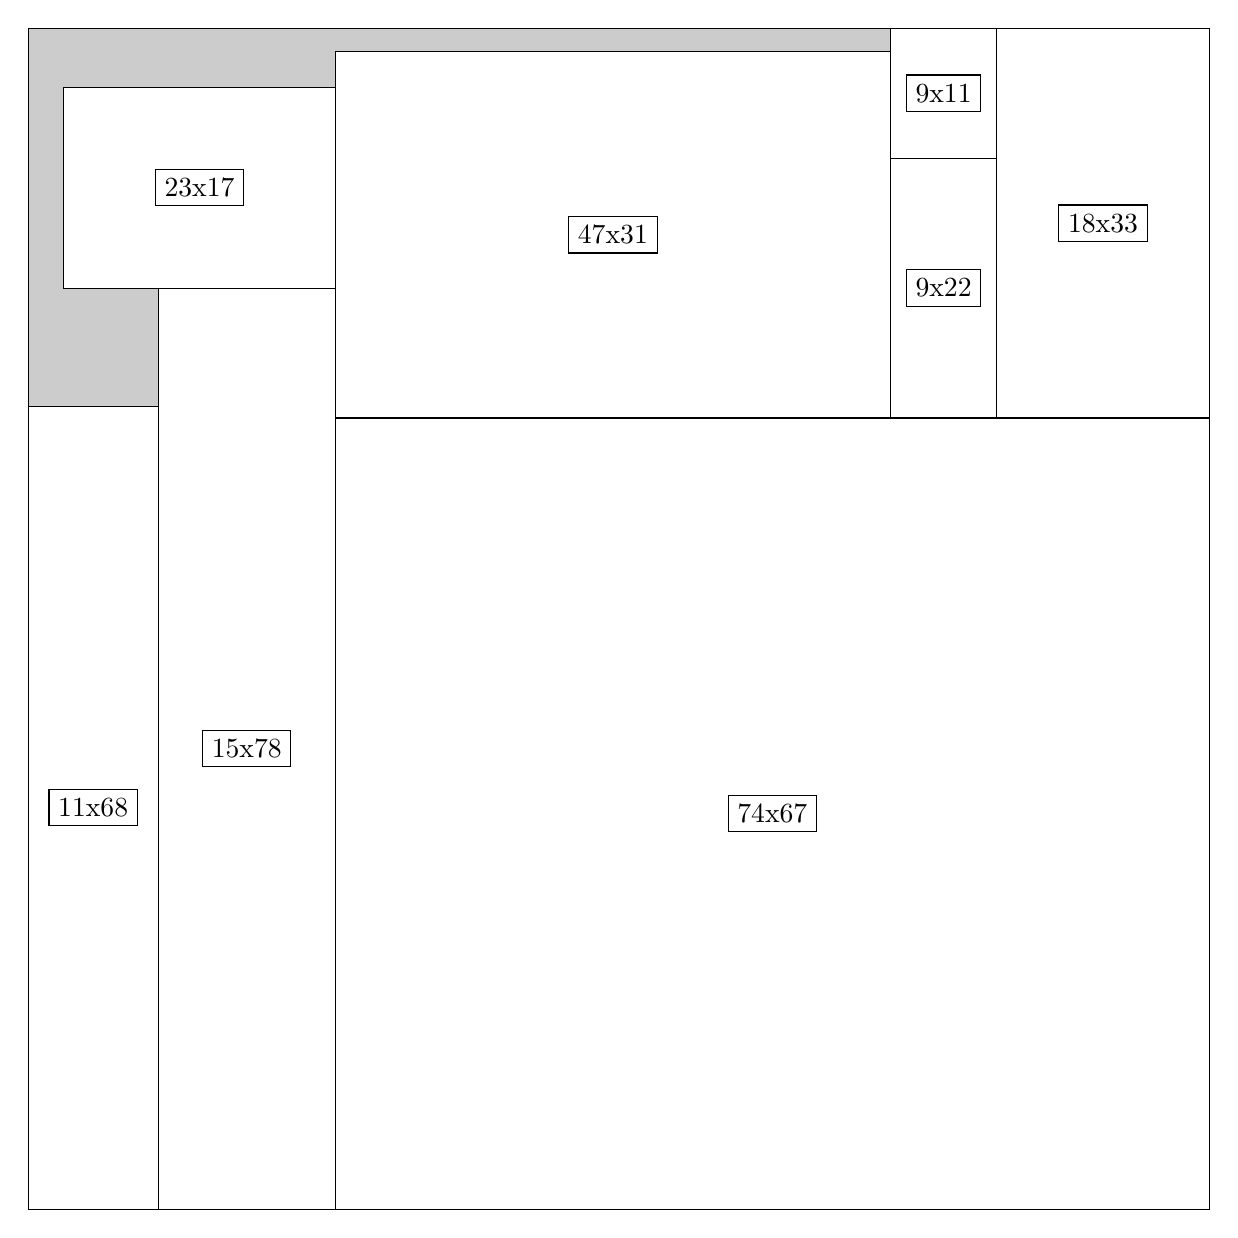
\begin{tikzpicture}[shorten >=1pt,scale=1.0,every node/.style={scale=1.0},->]
\tikzstyle{vertex}=[circle,fill=black!25,minimum size=14pt,inner sep=0pt]
\filldraw[fill=gray!40!white, draw=black] (0,0) rectangle (15.0,15.0);
\foreach \name/\x/\y/\w/\h in {74x67/3.9/0.0/11.1/10.049999999999999,18x33/12.299999999999999/10.049999999999999/2.6999999999999997/4.95,9x22/10.95/10.049999999999999/1.3499999999999999/3.3,9x11/10.95/13.35/1.3499999999999999/1.65,47x31/3.9/10.049999999999999/7.05/4.6499999999999995,15x78/1.65/0.0/2.25/11.7,11x68/0.0/0.0/1.65/10.2,23x17/0.44999999999999996/11.7/3.4499999999999997/2.55}
\filldraw[fill=white!40!white, draw=black] (\x,\y) rectangle node[draw] (\name) {\name} ++(\w,\h);
\end{tikzpicture}


w =74 , h =67 , x =26 , y =0 , v =4958
\par
w =18 , h =33 , x =82 , y =67 , v =594
\par
w =9 , h =22 , x =73 , y =67 , v =198
\par
w =9 , h =11 , x =73 , y =89 , v =99
\par
w =47 , h =31 , x =26 , y =67 , v =1457
\par
w =15 , h =78 , x =11 , y =0 , v =1170
\par
w =11 , h =68 , x =0 , y =0 , v =748
\par
w =23 , h =17 , x =3 , y =78 , v =391
\par
\newpage


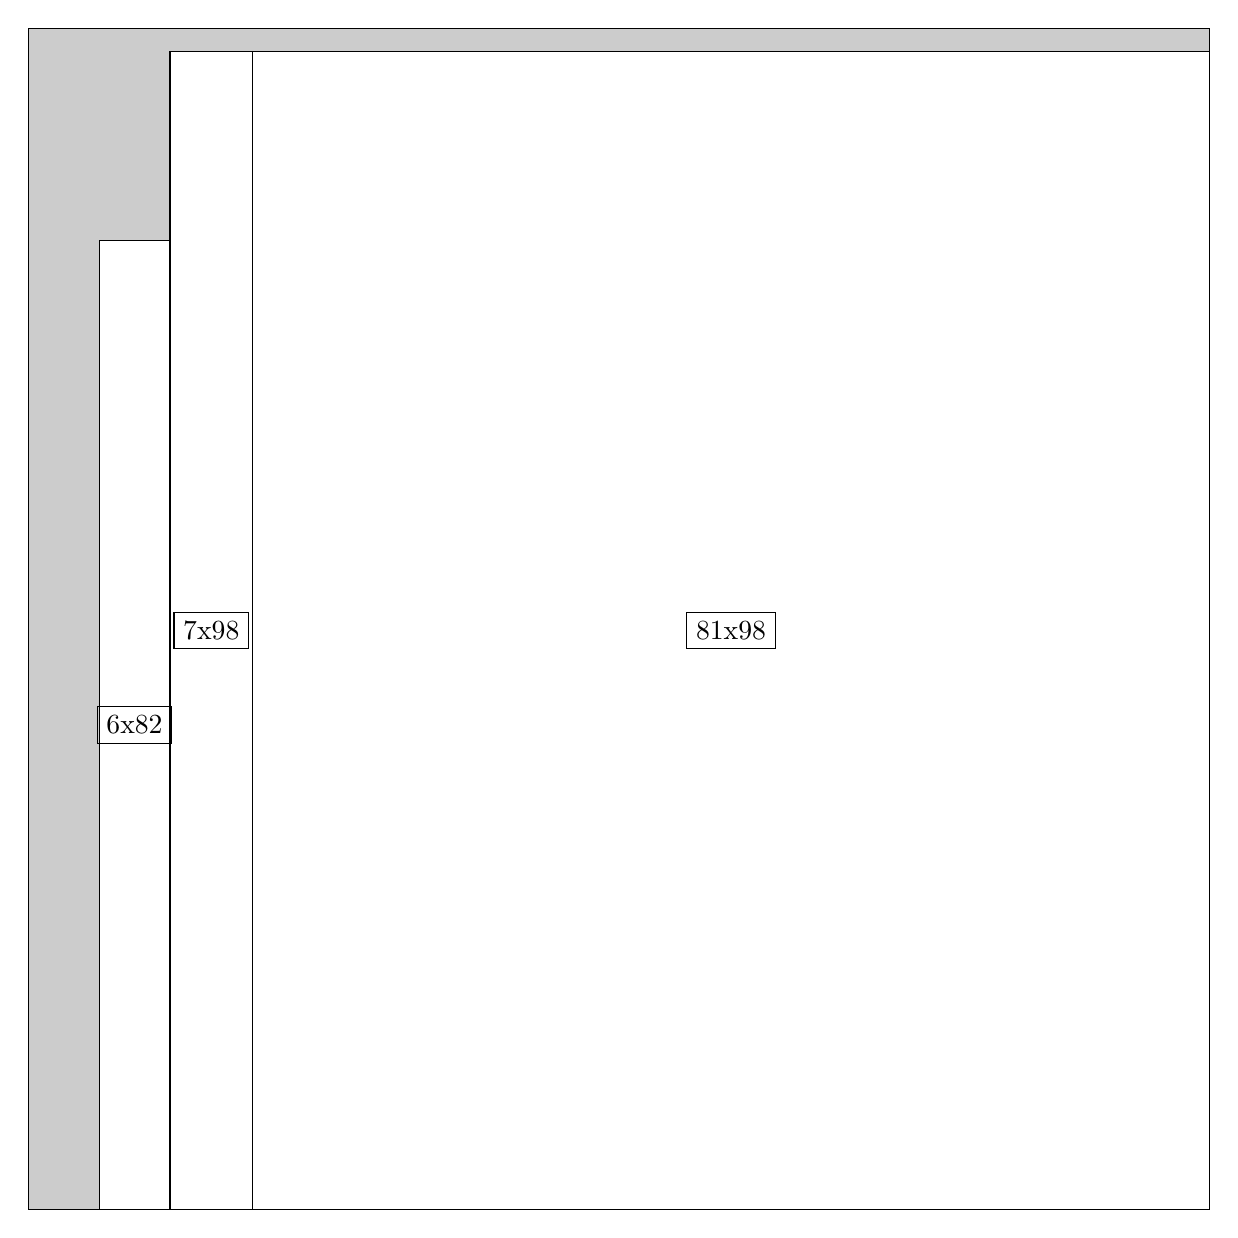
\begin{tikzpicture}[shorten >=1pt,scale=1.0,every node/.style={scale=1.0},->]
\tikzstyle{vertex}=[circle,fill=black!25,minimum size=14pt,inner sep=0pt]
\filldraw[fill=gray!40!white, draw=black] (0,0) rectangle (15.0,15.0);
\foreach \name/\x/\y/\w/\h in {81x98/2.85/0.0/12.15/14.7,7x98/1.7999999999999998/0.0/1.05/14.7,6x82/0.8999999999999999/0.0/0.8999999999999999/12.299999999999999}
\filldraw[fill=white!40!white, draw=black] (\x,\y) rectangle node[draw] (\name) {\name} ++(\w,\h);
\end{tikzpicture}


w =81 , h =98 , x =19 , y =0 , v =7938
\par
w =7 , h =98 , x =12 , y =0 , v =686
\par
w =6 , h =82 , x =6 , y =0 , v =492
\par
\newpage


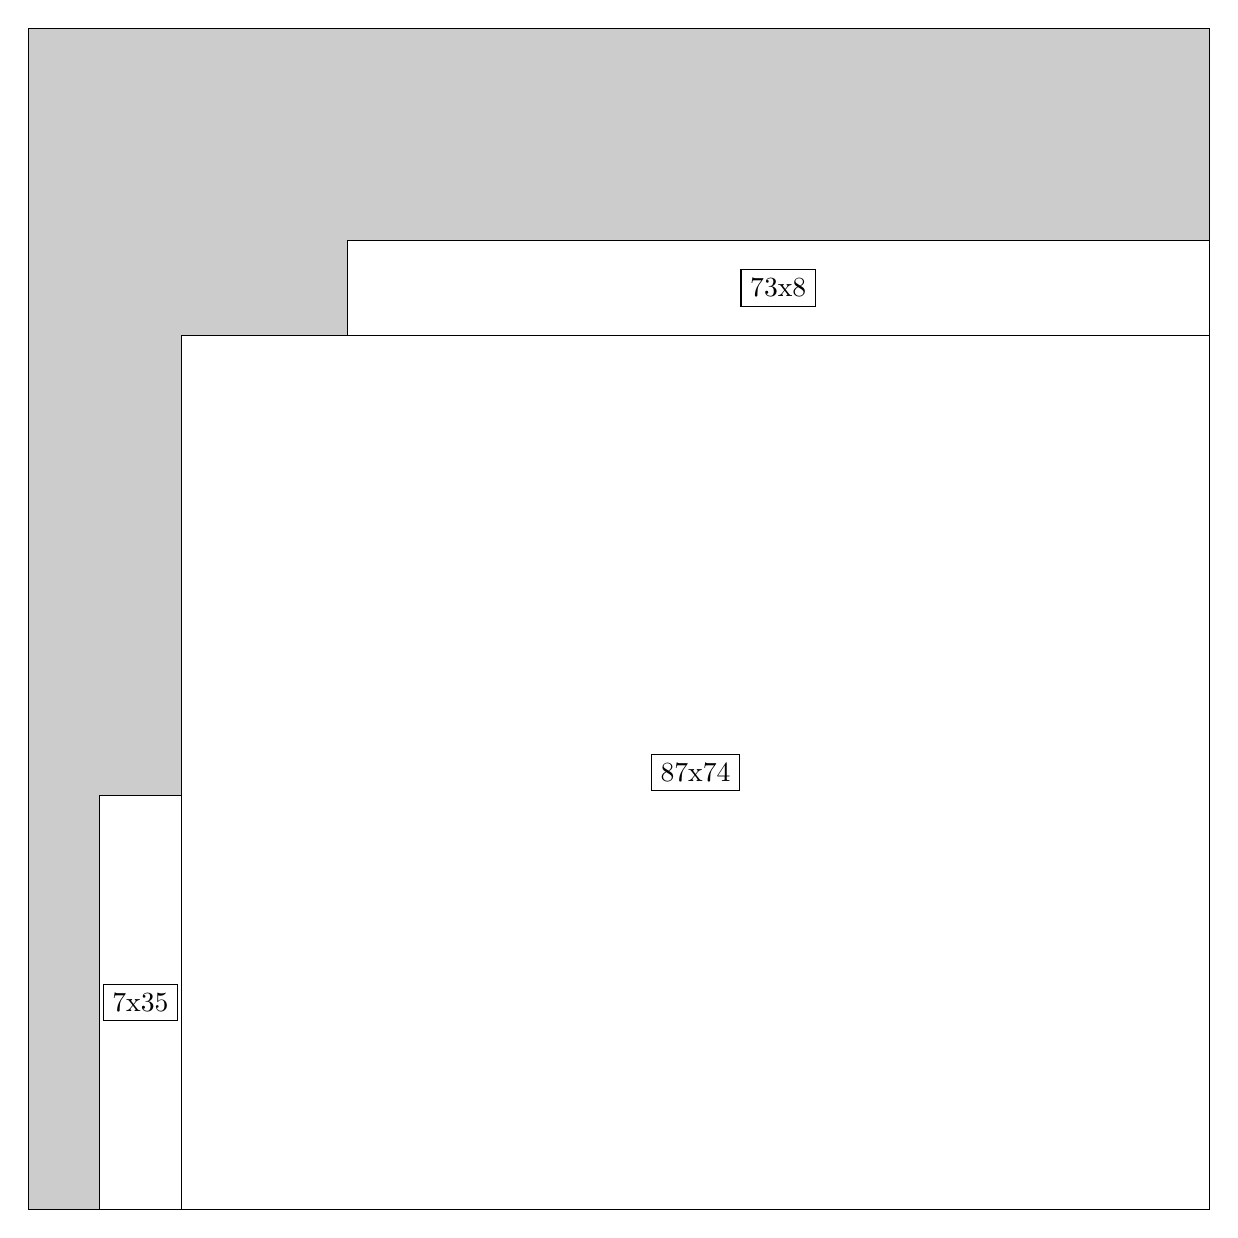
\begin{tikzpicture}[shorten >=1pt,scale=1.0,every node/.style={scale=1.0},->]
\tikzstyle{vertex}=[circle,fill=black!25,minimum size=14pt,inner sep=0pt]
\filldraw[fill=gray!40!white, draw=black] (0,0) rectangle (15.0,15.0);
\foreach \name/\x/\y/\w/\h in {87x74/1.95/0.0/13.049999999999999/11.1,7x35/0.8999999999999999/0.0/1.05/5.25,73x8/4.05/11.1/10.95/1.2}
\filldraw[fill=white!40!white, draw=black] (\x,\y) rectangle node[draw] (\name) {\name} ++(\w,\h);
\end{tikzpicture}


w =87 , h =74 , x =13 , y =0 , v =6438
\par
w =7 , h =35 , x =6 , y =0 , v =245
\par
w =73 , h =8 , x =27 , y =74 , v =584
\par
\newpage


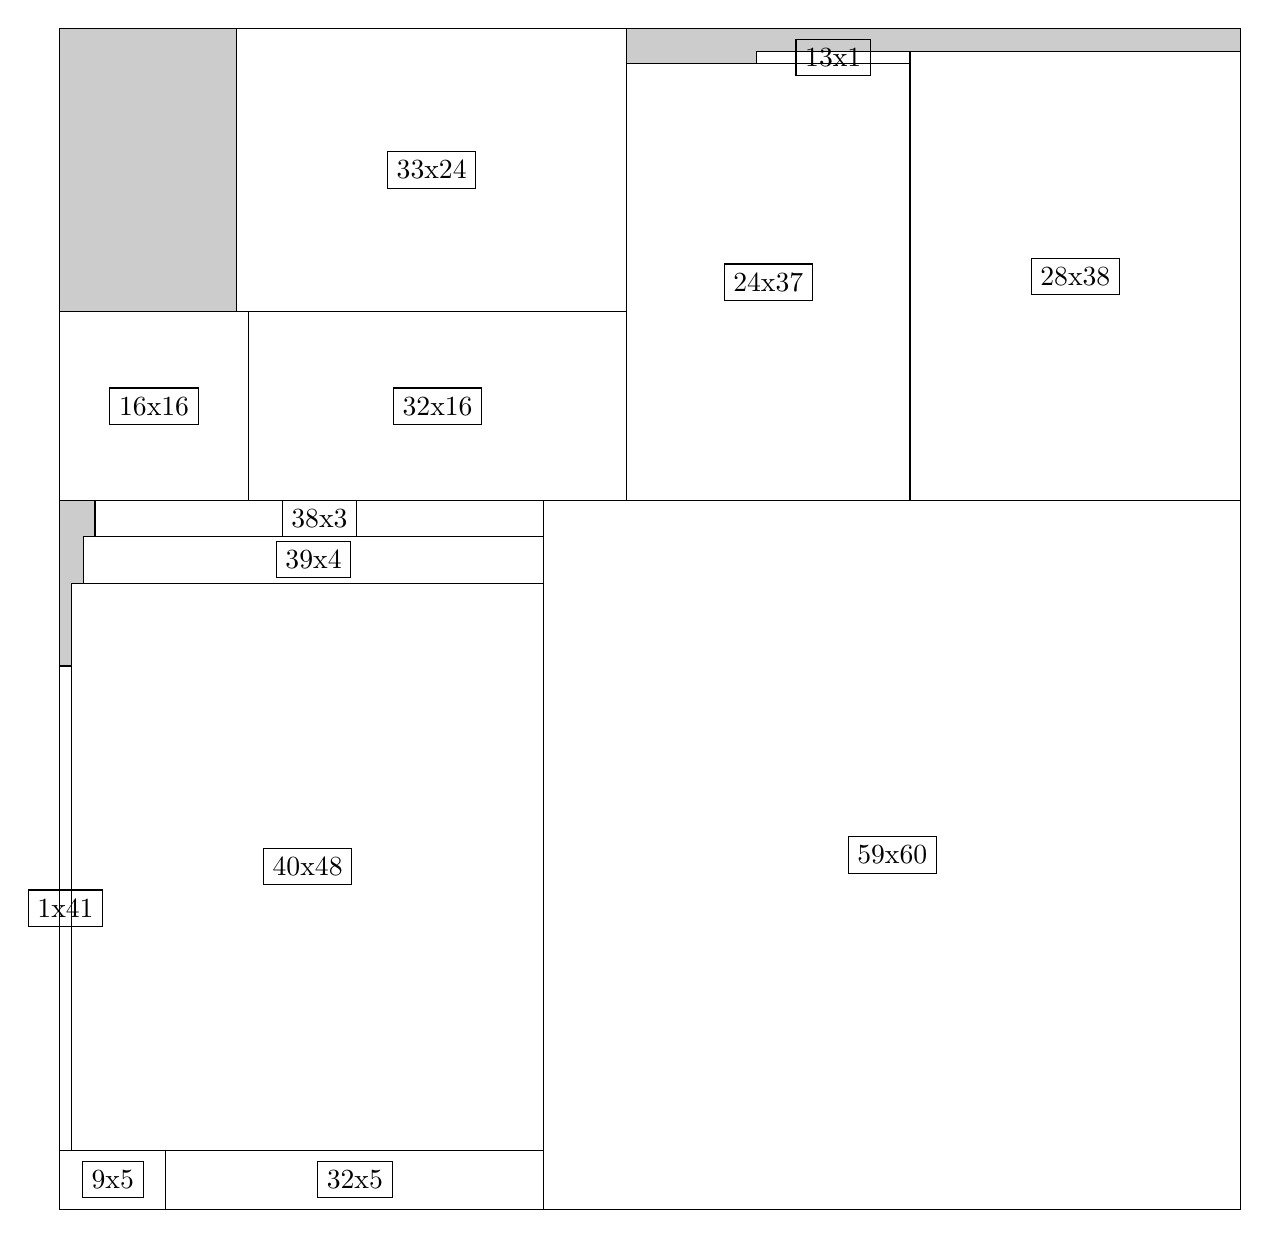
\begin{tikzpicture}[shorten >=1pt,scale=1.0,every node/.style={scale=1.0},->]
\tikzstyle{vertex}=[circle,fill=black!25,minimum size=14pt,inner sep=0pt]
\filldraw[fill=gray!40!white, draw=black] (0,0) rectangle (15.0,15.0);
\foreach \name/\x/\y/\w/\h in {59x60/6.1499999999999995/0.0/8.85/9.0,32x5/1.3499999999999999/0.0/4.8/0.75,9x5/0.0/0.0/1.3499999999999999/0.75,40x48/0.15/0.75/6.0/7.199999999999999,1x41/0.0/0.75/0.15/6.1499999999999995,39x4/0.3/7.949999999999999/5.85/0.6,38x3/0.44999999999999996/8.549999999999999/5.7/0.44999999999999996,28x38/10.799999999999999/9.0/4.2/5.7,24x37/7.199999999999999/9.0/3.5999999999999996/5.55,13x1/8.85/14.549999999999999/1.95/0.15,32x16/2.4/9.0/4.8/2.4,16x16/0.0/9.0/2.4/2.4,33x24/2.25/11.4/4.95/3.5999999999999996}
\filldraw[fill=white!40!white, draw=black] (\x,\y) rectangle node[draw] (\name) {\name} ++(\w,\h);
\end{tikzpicture}


w =59 , h =60 , x =41 , y =0 , v =3540
\par
w =32 , h =5 , x =9 , y =0 , v =160
\par
w =9 , h =5 , x =0 , y =0 , v =45
\par
w =40 , h =48 , x =1 , y =5 , v =1920
\par
w =1 , h =41 , x =0 , y =5 , v =41
\par
w =39 , h =4 , x =2 , y =53 , v =156
\par
w =38 , h =3 , x =3 , y =57 , v =114
\par
w =28 , h =38 , x =72 , y =60 , v =1064
\par
w =24 , h =37 , x =48 , y =60 , v =888
\par
w =13 , h =1 , x =59 , y =97 , v =13
\par
w =32 , h =16 , x =16 , y =60 , v =512
\par
w =16 , h =16 , x =0 , y =60 , v =256
\par
w =33 , h =24 , x =15 , y =76 , v =792
\par
\newpage


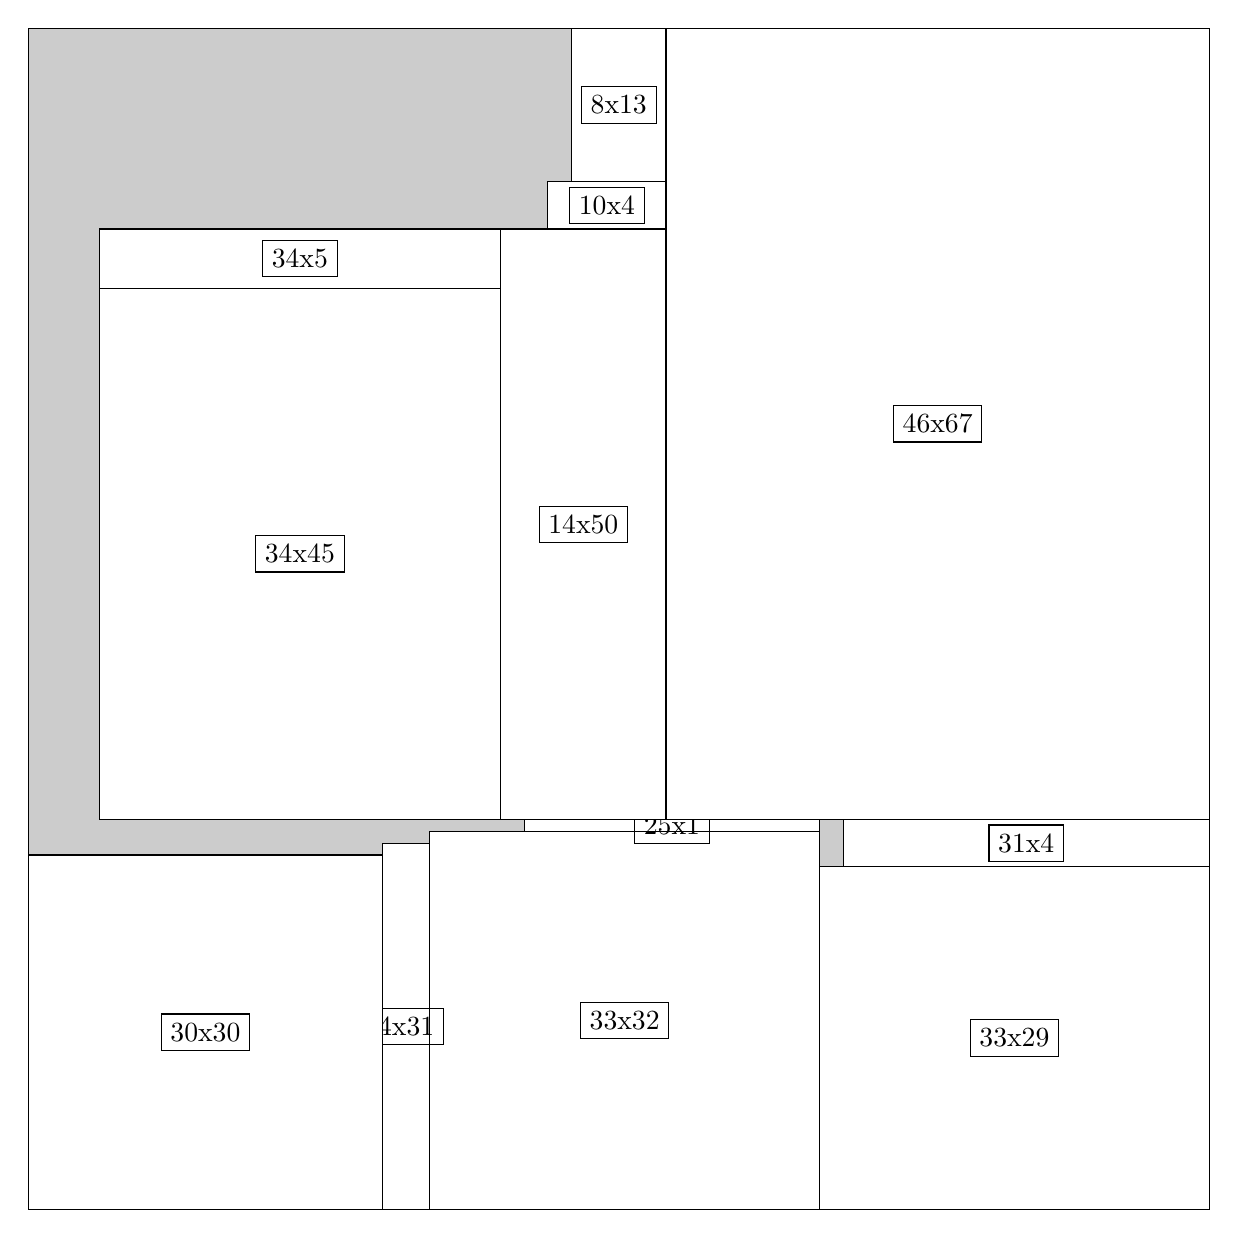
\begin{tikzpicture}[shorten >=1pt,scale=1.0,every node/.style={scale=1.0},->]
\tikzstyle{vertex}=[circle,fill=black!25,minimum size=14pt,inner sep=0pt]
\filldraw[fill=gray!40!white, draw=black] (0,0) rectangle (15.0,15.0);
\foreach \name/\x/\y/\w/\h in {33x29/10.049999999999999/0.0/4.95/4.35,31x4/10.35/4.35/4.6499999999999995/0.6,33x32/5.1/0.0/4.95/4.8,25x1/6.3/4.8/3.75/0.15,4x31/4.5/0.0/0.6/4.6499999999999995,30x30/0.0/0.0/4.5/4.5,46x67/8.1/4.95/6.8999999999999995/10.049999999999999,14x50/6.0/4.95/2.1/7.5,10x4/6.6/12.45/1.5/0.6,8x13/6.8999999999999995/13.049999999999999/1.2/1.95,34x45/0.8999999999999999/4.95/5.1/6.75,34x5/0.8999999999999999/11.7/5.1/0.75}
\filldraw[fill=white!40!white, draw=black] (\x,\y) rectangle node[draw] (\name) {\name} ++(\w,\h);
\end{tikzpicture}


w =33 , h =29 , x =67 , y =0 , v =957
\par
w =31 , h =4 , x =69 , y =29 , v =124
\par
w =33 , h =32 , x =34 , y =0 , v =1056
\par
w =25 , h =1 , x =42 , y =32 , v =25
\par
w =4 , h =31 , x =30 , y =0 , v =124
\par
w =30 , h =30 , x =0 , y =0 , v =900
\par
w =46 , h =67 , x =54 , y =33 , v =3082
\par
w =14 , h =50 , x =40 , y =33 , v =700
\par
w =10 , h =4 , x =44 , y =83 , v =40
\par
w =8 , h =13 , x =46 , y =87 , v =104
\par
w =34 , h =45 , x =6 , y =33 , v =1530
\par
w =34 , h =5 , x =6 , y =78 , v =170
\par
\newpage


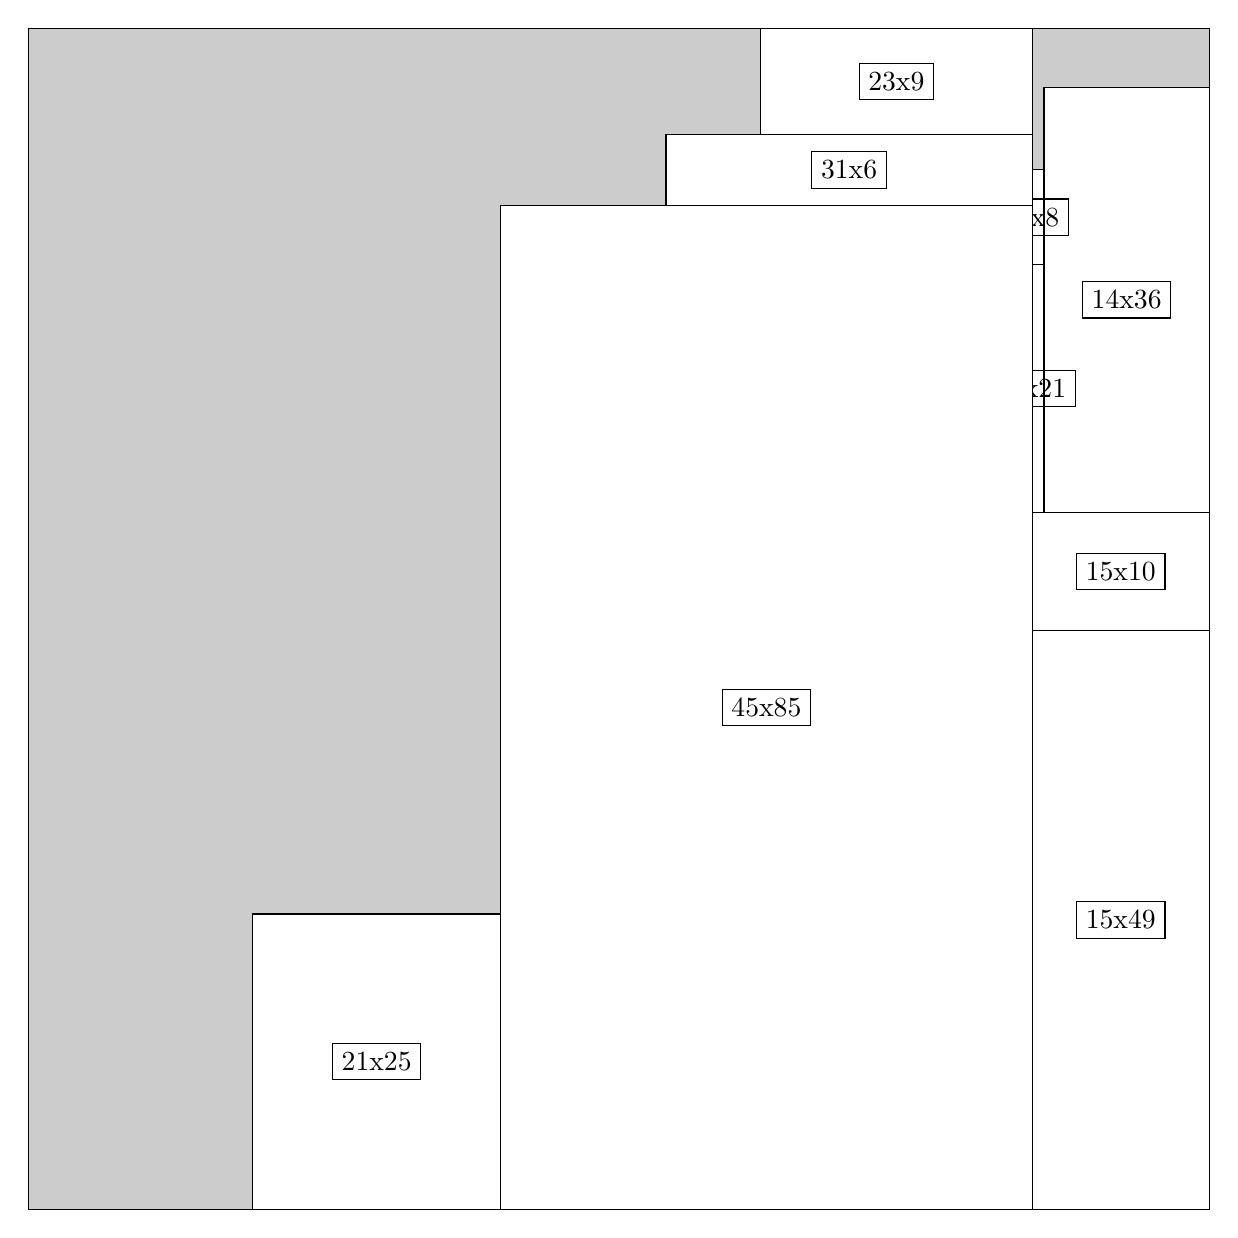
\begin{tikzpicture}[shorten >=1pt,scale=1.0,every node/.style={scale=1.0},->]
\tikzstyle{vertex}=[circle,fill=black!25,minimum size=14pt,inner sep=0pt]
\filldraw[fill=gray!40!white, draw=black] (0,0) rectangle (15.0,15.0);
\foreach \name/\x/\y/\w/\h in {15x49/12.75/0.0/2.25/7.35,15x10/12.75/7.35/2.25/1.5,14x36/12.9/8.85/2.1/5.3999999999999995,1x21/12.75/8.85/0.15/3.15,1x8/12.75/12.0/0.15/1.2,45x85/6.0/0.0/6.75/12.75,31x6/8.1/12.75/4.6499999999999995/0.8999999999999999,23x9/9.299999999999999/13.65/3.4499999999999997/1.3499999999999999,21x25/2.85/0.0/3.15/3.75}
\filldraw[fill=white!40!white, draw=black] (\x,\y) rectangle node[draw] (\name) {\name} ++(\w,\h);
\end{tikzpicture}


w =15 , h =49 , x =85 , y =0 , v =735
\par
w =15 , h =10 , x =85 , y =49 , v =150
\par
w =14 , h =36 , x =86 , y =59 , v =504
\par
w =1 , h =21 , x =85 , y =59 , v =21
\par
w =1 , h =8 , x =85 , y =80 , v =8
\par
w =45 , h =85 , x =40 , y =0 , v =3825
\par
w =31 , h =6 , x =54 , y =85 , v =186
\par
w =23 , h =9 , x =62 , y =91 , v =207
\par
w =21 , h =25 , x =19 , y =0 , v =525
\par
\newpage


\end{document}